\chapter{Software implementation}
\label{Software}
% \minitoc
% 

\includegraphics[width=.075\textwidth]{gfx/Scihub_raven.png}
\cleanchapterquote{Journal paywalls are an example of something that works in the reverse direction, making communication less open and efficient.}{Alexandra Elbakyan}{}
% 
% \tikz[remember picture,overlay] \node[inner sep=0pt] at (0,0){
\includegraphics[height=7em]{gfx/Scihub_raven.png}};
% \hspace{-10em}

% \clearpage opacity=0.3,
% 
\comment{\paragraph{Ziele:} 
\begin{itemize}
    \item User-Friendly: Python
    \item ... C++
    \item 
\end{itemize}}
%
\cite{pybind11}

\section{Introduction}

\section{Framework}
The software package \ac{fastPLI} is build as a \textit{Python3} \cite{Python3} package.

To explain Python packages, first Python modules needs to be explained.

Simply said, a Python module is a collection of executable functions. They can however also contain other modules. Their structure is exacly build up like a file structure. 

A Python package on the other side is a collection of python code and modules. Their sturcture are indistinguishable from modules, however they contain additional instruction for the installation process. E.g Python can also run compiled shared \CCXX{} functions. A python package can include the instructions to compile this functions with a suitable \CCXX{} compiler and a list of all necessary additional \CCXX{}-Libraries.

\begin{figure}
    \centering
    % \resizebox{1.0\textwidth}{!}{
    \begin{tabular}{lr}
    \begin{minipage}[t]{0.45\textwidth}
    \dirtree{%
        % .1 \_\_init\_\_.py.
        .1 analysis.
        .2 \_\_init\_\_.py.
        .2 \_ROFL\_with\_jacobi.py.
        .2 affine\_transformation.py.
        .2 epa.py.
        .2 images.py.
        .2 rofl.py.
    }
    \vspace{1em}
    \dirtree{%
        .1 io.
        .2 \_\_init\_\_.py.
        .2 fiber.py.
    }
    \vspace{1em}
    \dirtree{%
        .1 model.
        .2 \_\_init\_\_.py.
        .2 \_visualizer.py.
        .2 sandbox.
        .3 \_\_init\_\_.py.
        .3 fill.py.
        .3 shape.py.
        .2 solver.
        .3 \_\_init\_\_.py.
        .3 \_\_solver.cpython.so.
        .3 \_solver.py.
    }
    \end{minipage}
    &
    \begin{minipage}[t]{0.45\textwidth}
    \dirtree{%
        .1 objects.
        .2 \_\_init\_\_.py.
        .2 fiber.py.
        .2 fiber\_bundle.py.
        .2 fiber\_bundles.py.
    }
    \vspace{1em}
    \dirtree{%
        .1 simulation.
        .2 \_\_init\_\_.py.
        .2 \_\_generation.cpython.so.
        .2 \_\_simulation.cpython.so.
        .2 \_simpli.py.
        .2 optic.py.
    }
    \vspace{1em}
    \dirtree{%
        .1 tools.
        .2 \_\_init\_\_.py.
        .2 label\_converter.py.
        .2 rotation.py.
        % .1 version.py.
        }
    \end{minipage}
    \\
    \end{tabular}
    % }
    \caption{package dirlist, see \dummy.} %\cref{app:fastpli}
    \label{fig:package_dirlist}
\end{figure}


\subsection{Dependencies}
% 
\paragraph{Python:}
\begin{description}
\item[numpy:] Base N-dimensional array package \cite{2019arXiv190710121V}\\
\url{https://numpy.org/}
\item[scipy:] Fundamental library for scientific computing \cite{2019arXiv190710121V}\\
\url{https://www.scipy.org/} 
\item[numba:] Acceleration of Python Functions \cite{Lam2015}\\
\url{https://numba.pydata.org/}
\item[mpi4py:] MPI for Python \cite{Dalcn2005, Dalcn2008, Dalcin2011}\\
\url{https://bitbucket.org/mpi4py/mpi4py/src/master/}
\item[h5py:] HDF5 for Python \cite{collette_python_hdf5_2014, hdf5}\\
\url{https://www.h5py.org/}
\end{description}
% 
\paragraph{C++:}
\begin{description}
\item[MPI:] Message Passing Interface \cite{message2015mpi}\\
\url{https://www.mpi-forum.org/}
\item[OpenMP:] Open Multi-Processing, API for multi-platform shared memory multiprocessing programming \cite{dagum1998openmp}\\
\url{https://www.openmp.org/}
\item[OpenGL:] Open Graphics Library \cite{khronos}\\
\url{www.opengl.org}
\item[Pybind11:] Seamless operability between C++11 and Python \cite{pybind11}\\ \url{https://github.com/pybind/pybind11} 
\end{description}


\begin{figure}[!tb]
\centering
\resizebox{0.95\textwidth}{!}{
 \inputtikz{gfx/fastpli/fastpli_sim_pipeline.tikz}}
\caption{pipeline}
\label{fig:sim_pipeline}
\end{figure}
% 
\begin{figure}[!tb]
    \centering
    \fbox{
    \resizebox{0.95\textwidth}{!}{
    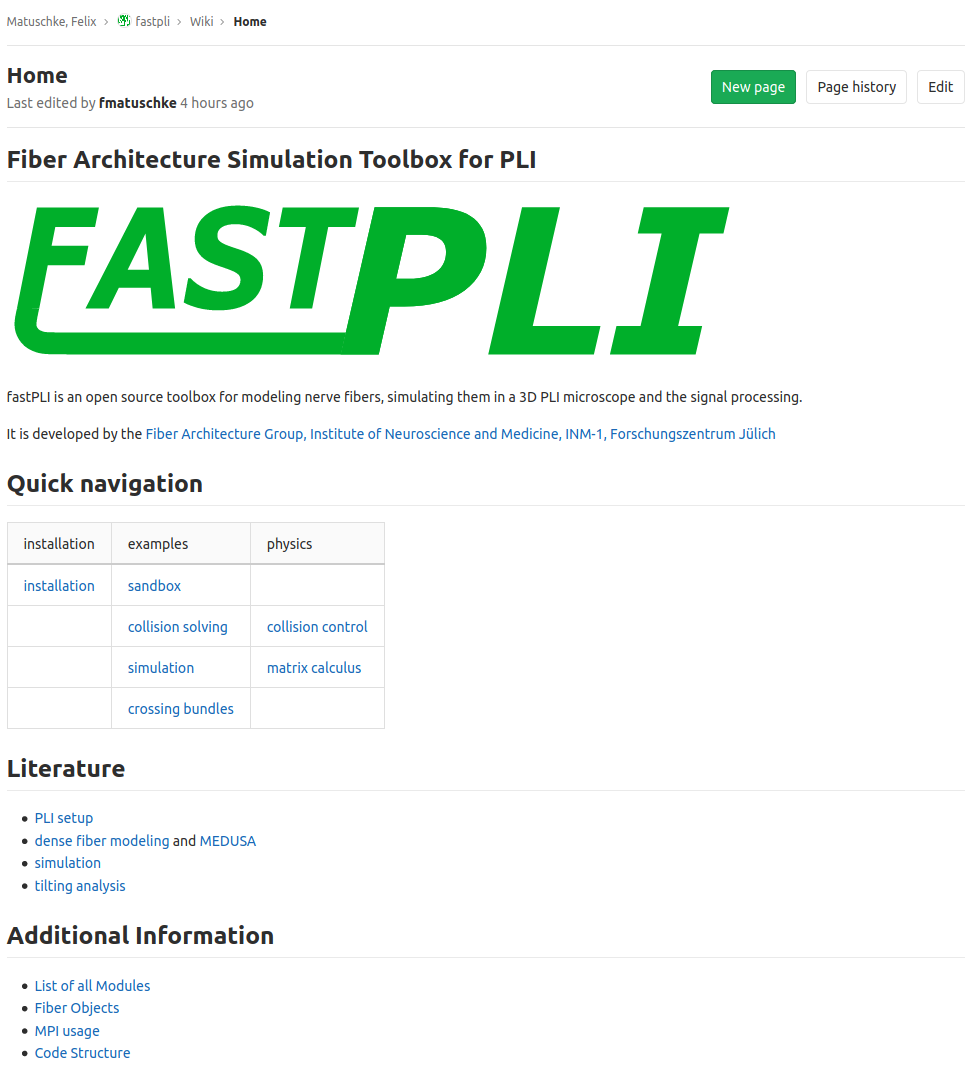
\includegraphics[width=0.95\textwidth,height=0.95\textheight,keepaspectratio,trim={400px 42px 460px 42px},clip]{gfx/fastpli/fastpli_wiki_home.png}}}
	\caption{dummy}
	\label{fig:fastpli_wiki_home}
\end{figure}
% 
\begin{figure}[!tb]
    \centering
    \fbox{
    \resizebox{0.95\textwidth}{!}{
    \begin{tabular}{c|c}
         	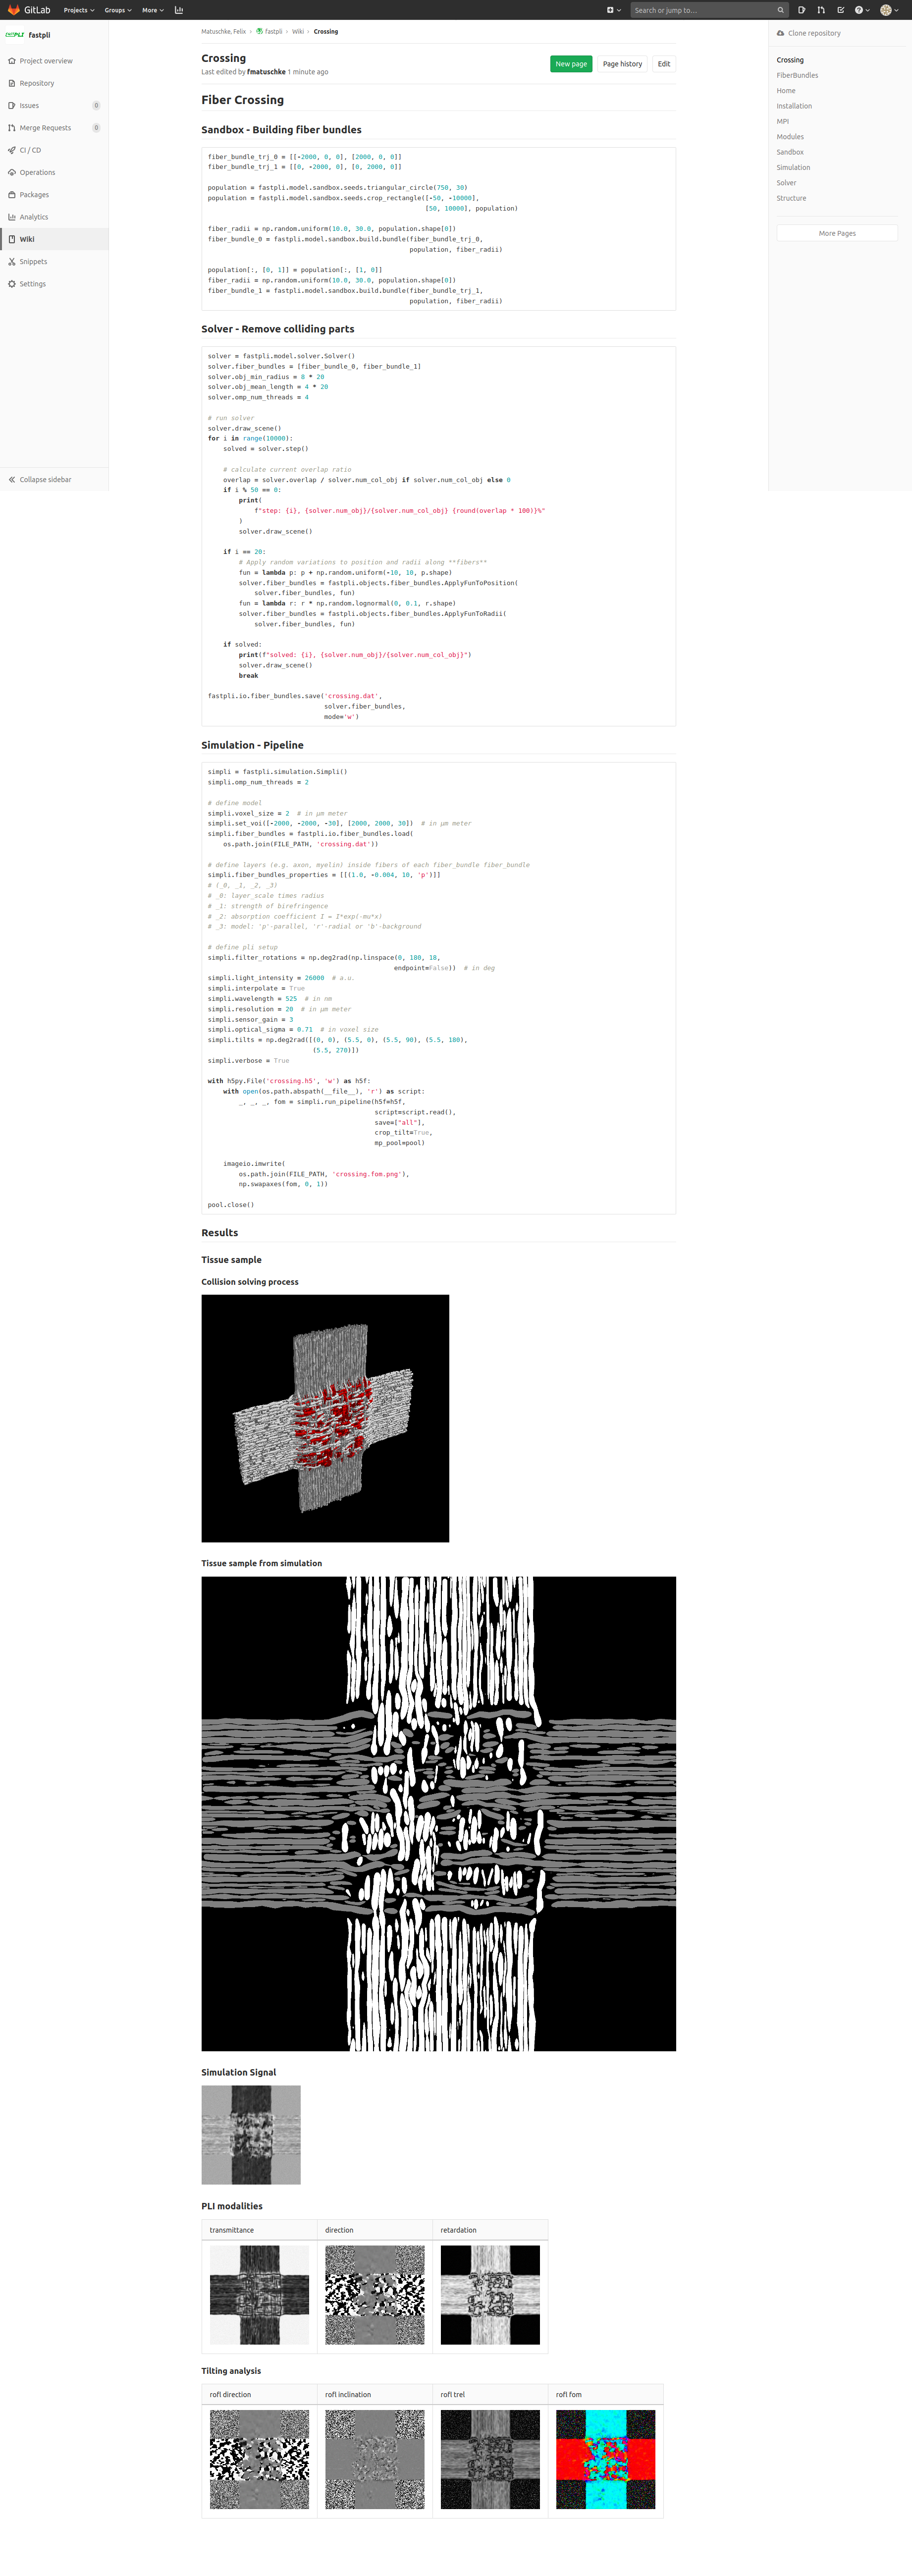
\includegraphics[width=\textwidth,height=\textheight,keepaspectratio,
         					trim={400px 2735px 460px 42px},clip]{
         						gfx/fastpli/fastpli_wiki_crossing.png} &
         	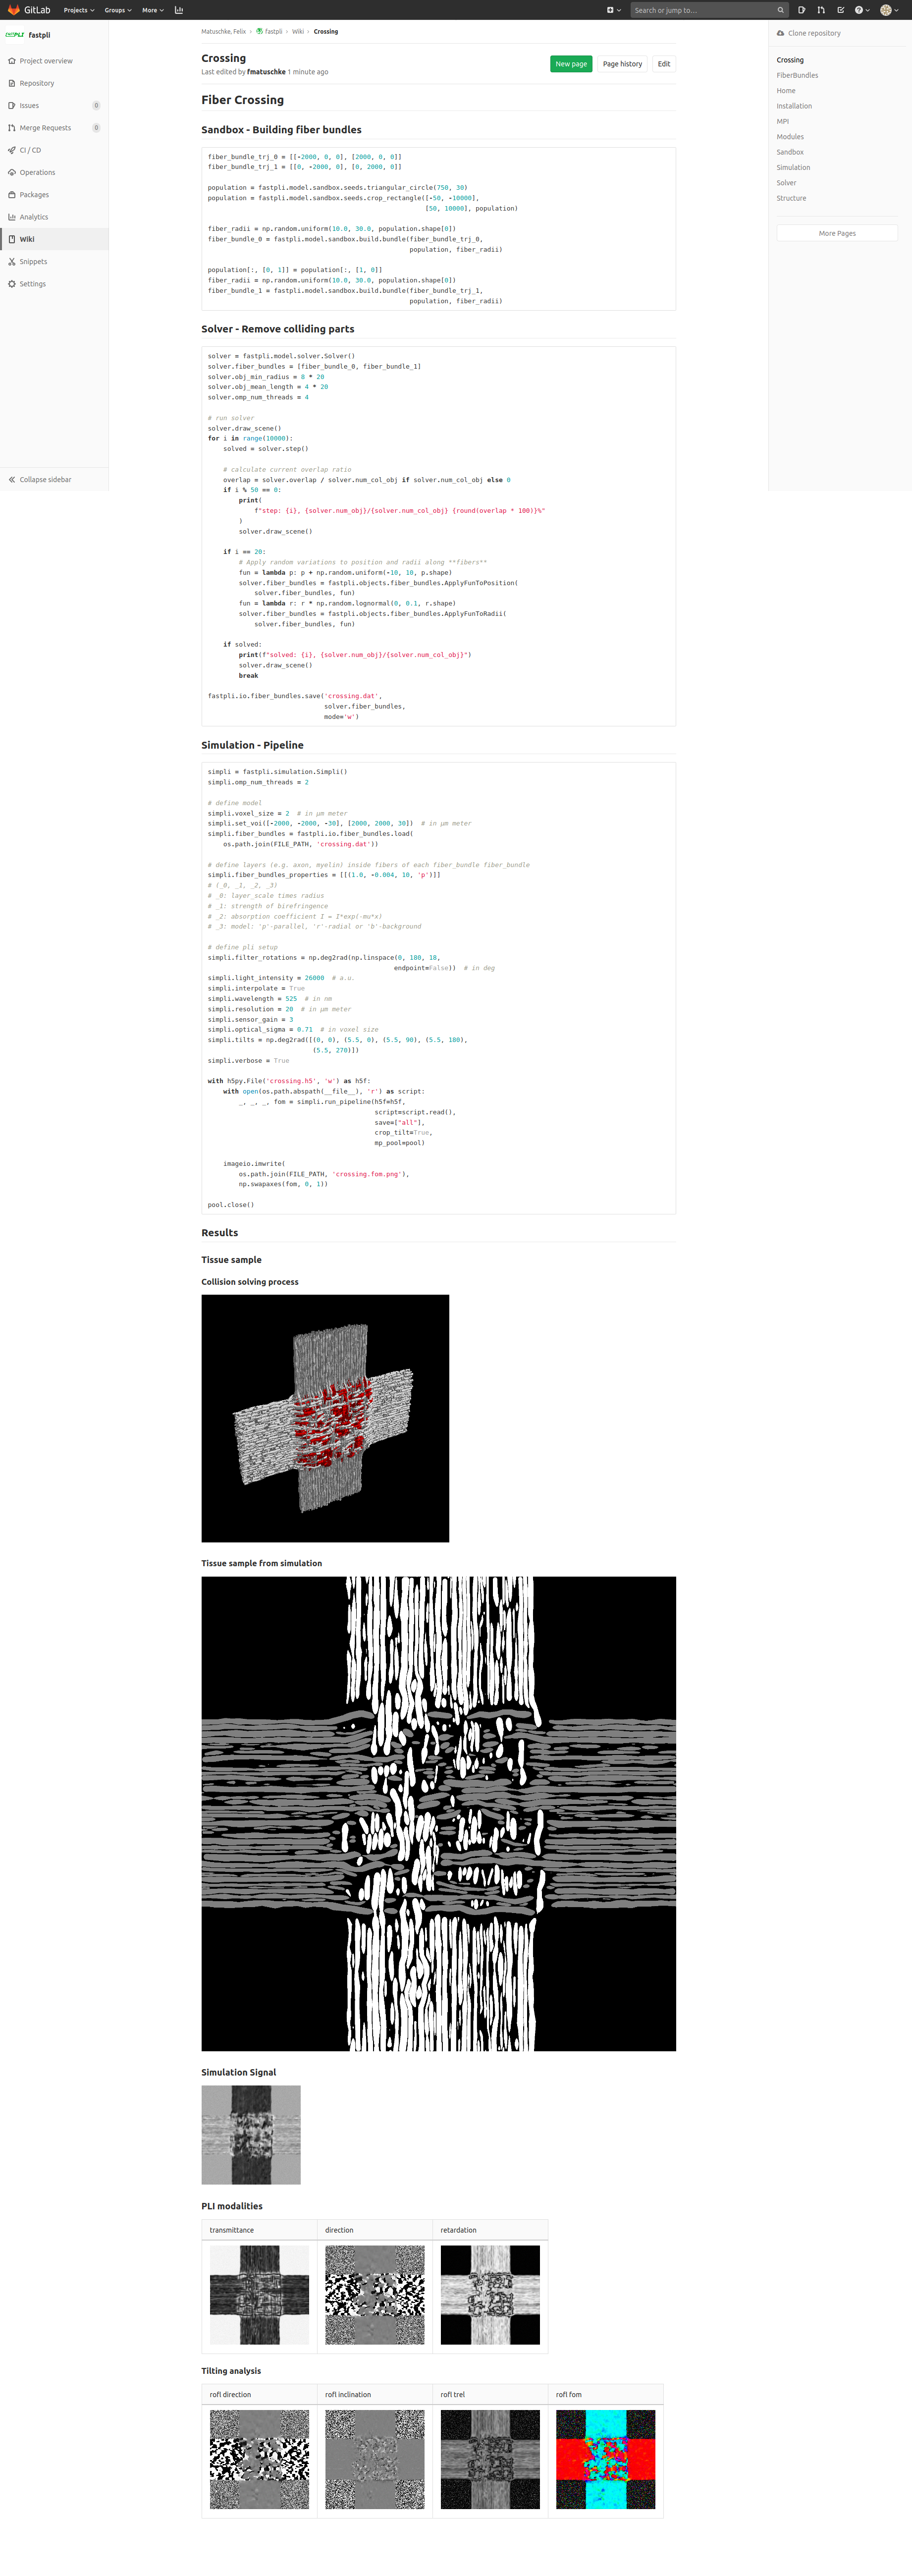
\includegraphics[width=\textwidth,height=\textheight,keepaspectratio,
         					trim={400px 42px 460px 2465px},clip]{
         						gfx/fastpli/fastpli_wiki_crossing.png}  \\
    \end{tabular}
    }}
	\caption{dummy}
	\label{fig:fastpli_wiki_crossing}
\end{figure}
% 
% 
% A Python packages is a seperated into \textit{modules}.
% A Python packages is the overhaul collection of all modules and instructions.
% Models  \begin{quote}
%     A module can contain executable statements as well as function definitions. [\,\dots] Modules can import other modules.
% \end{quote}

% \begin{figure}[!h]
% \begin{lstlisting}[language=python]
% import my-package.my-module
% \end{lstlisting}
% \label{fig:python_test}
% \caption{python test.}
% \end{figure}


%
%\begin{figure}[!tb]
%	\centering
%	\resizebox{\textwidth}{!}{
%		\tikzfigure{mindmap}
%	}
%	\label{fig:mindmap}
%	\caption{mindmap.}
%\end{figure}
%
% \begin{figure}
% 	\centering
% 	\resizebox{\textwidth}{!}{
% 	\tikzfigure{uml-example}
% 	}
% \end{figure}
%
% \begin{figure}[!tb]
% 	\centering
% 	\resizebox{\textwidth}{!}{
% 		\inputtikz{gfx/fastpli/fastpli_diagram.tikz}
% 	}
% 	\label{fig:fastpli_diagram}
% 	\caption{fastpli diagram.}
% \end{figure}
%
% \begin{figure}[!tb]
% 	\lstinputlisting[language=python]{code/dummy.py}
% 	\label{fig:python_test}
% 	\caption{python test.}
% \end{figure}
%
%
